\begin{frame}
  \frametitle{Anisotropies in the CMB}
  \framesubtitle{A more interesting picture}

  \begin{overlayarea}{\textwidth}{\textheight}

    \only<1-2>{%
      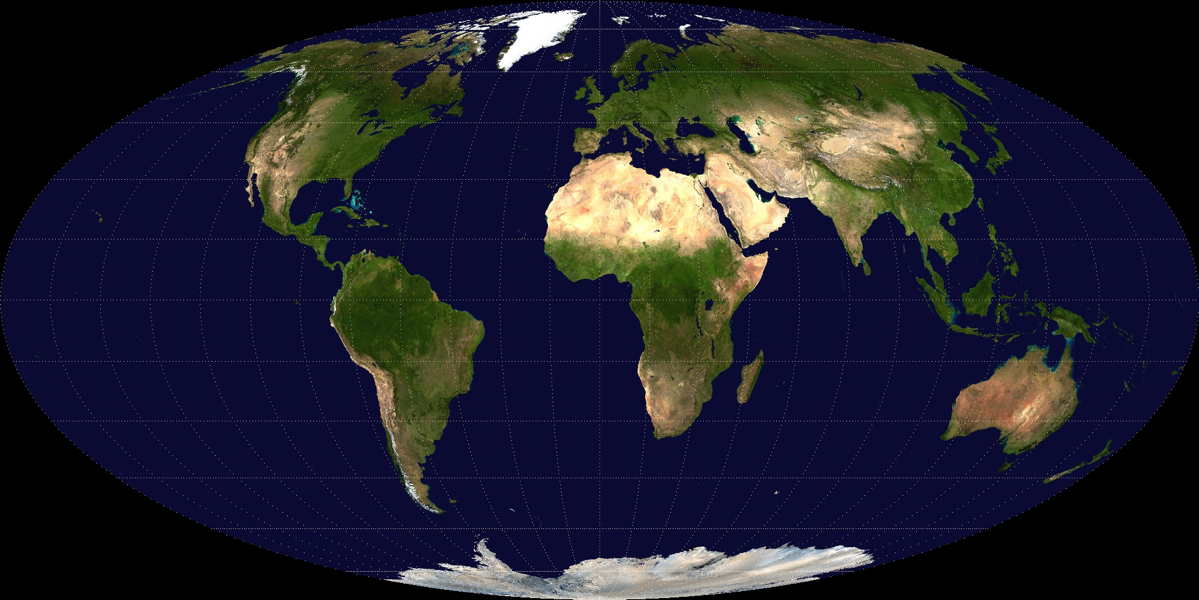
\includegraphics[width=\textwidth]{Images/Mollweide-projection.png}
    }
    \only<3-4>{%
      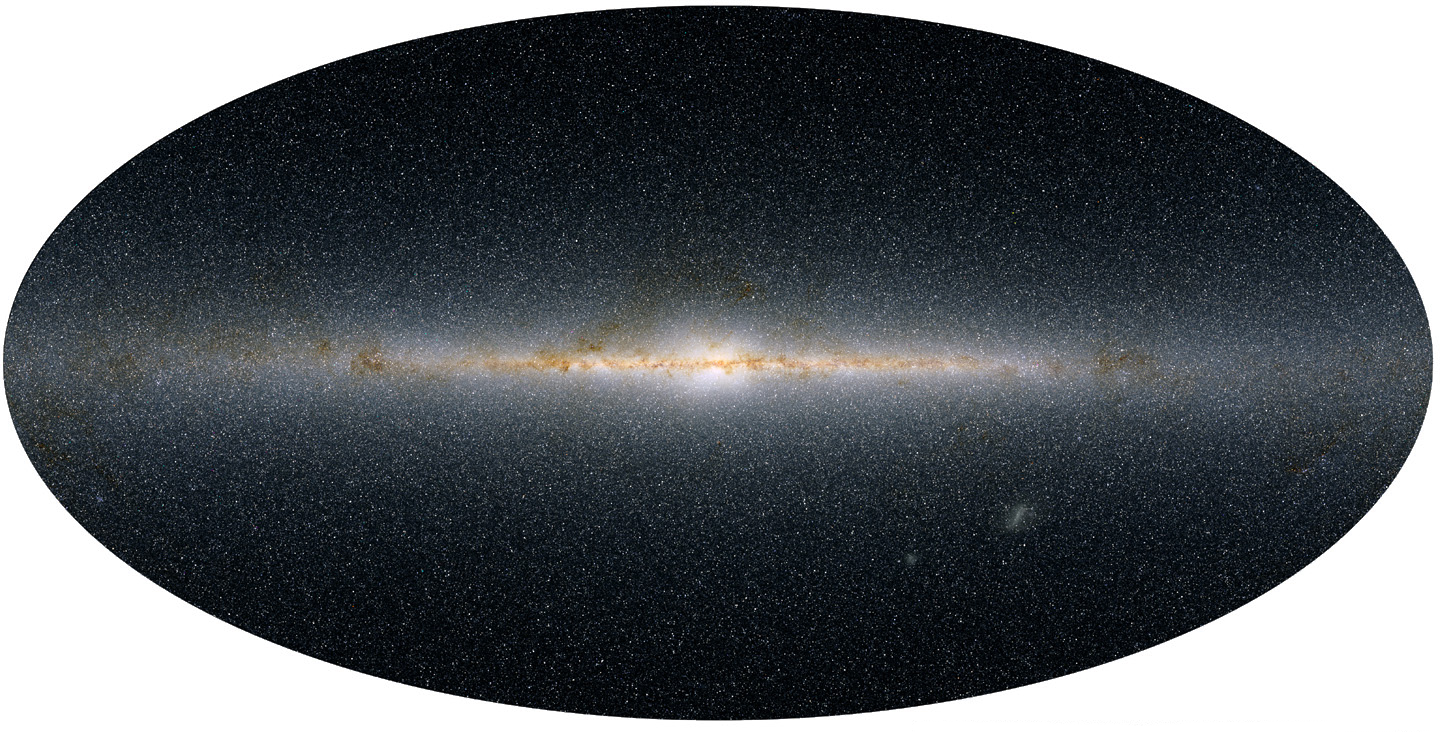
\includegraphics[width=\textwidth]{Images/Milky_Way_infrared.png}
    }
    \only<5-6>{%
      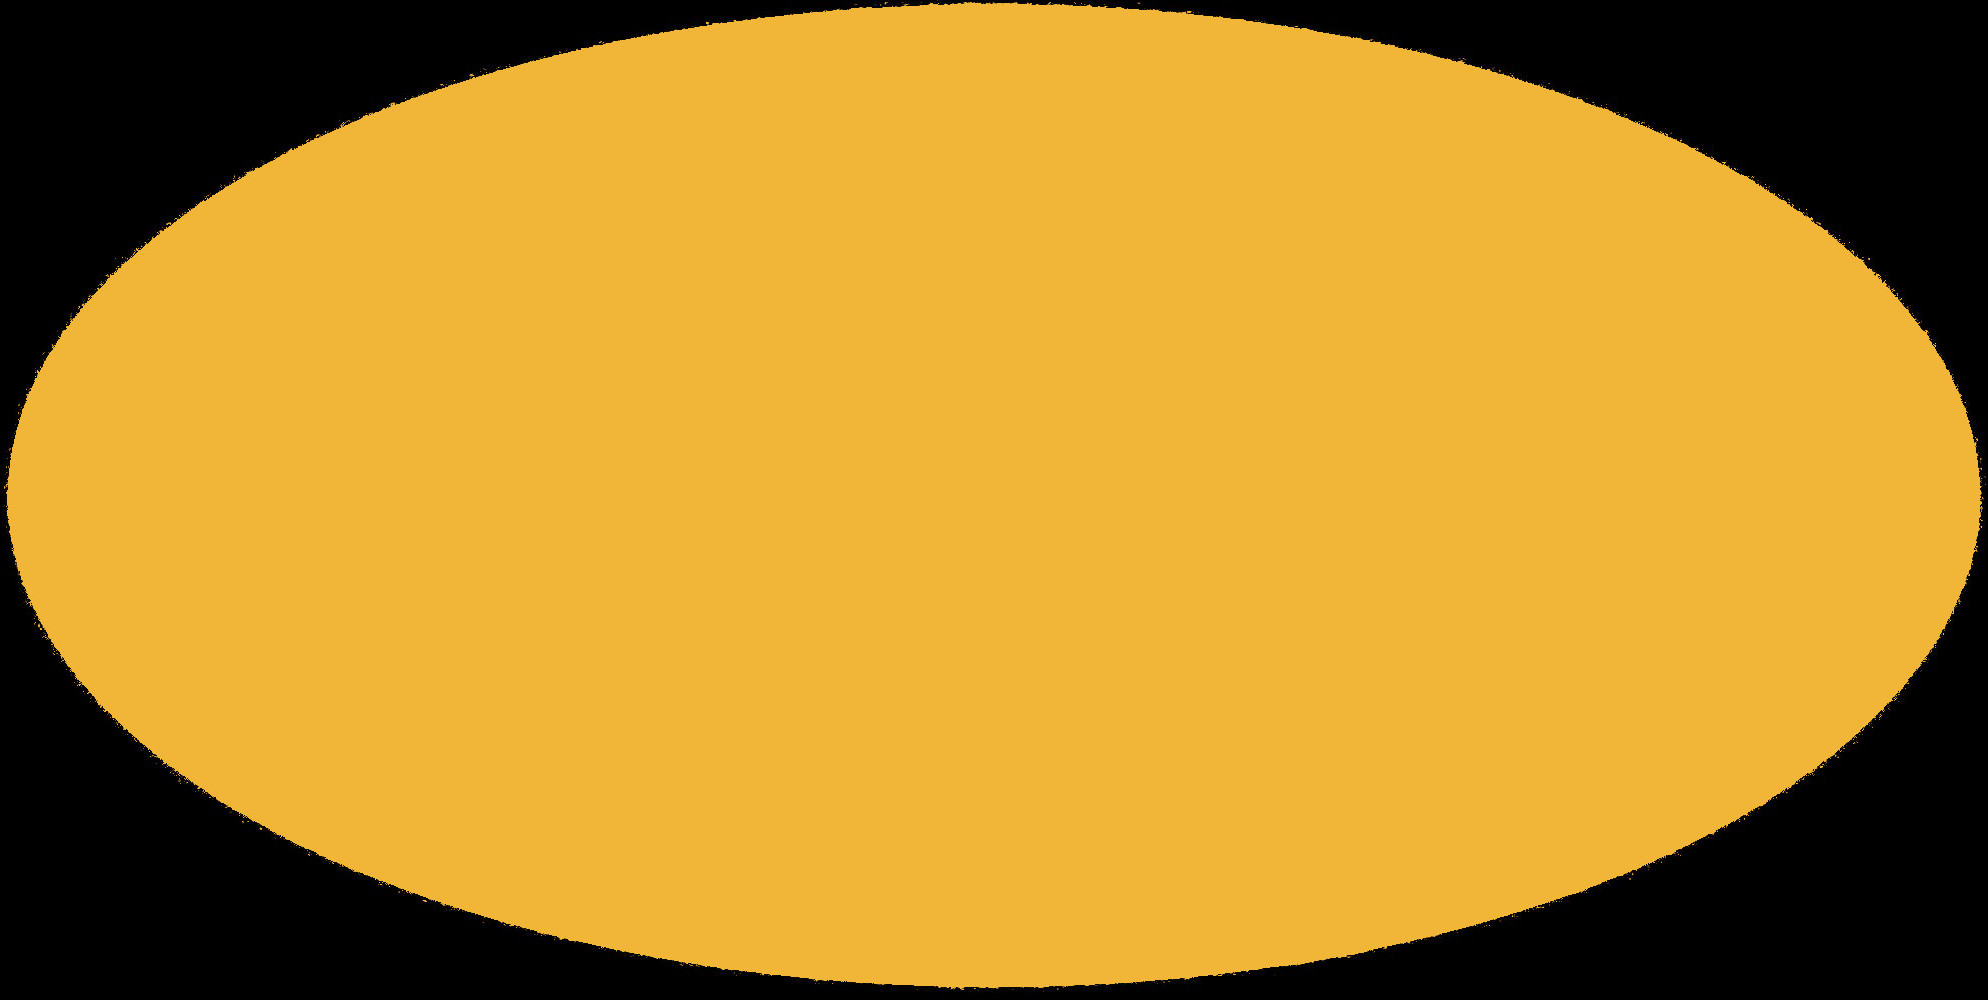
\includegraphics[width=\textwidth]{Images/monopole.jpg}
    }
    \only<7-12>{%
      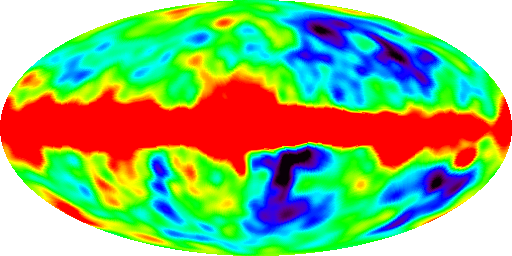
\includegraphics[width=\textwidth]{Images/cobe_1.png}
    }
    \only<13-13>{%
      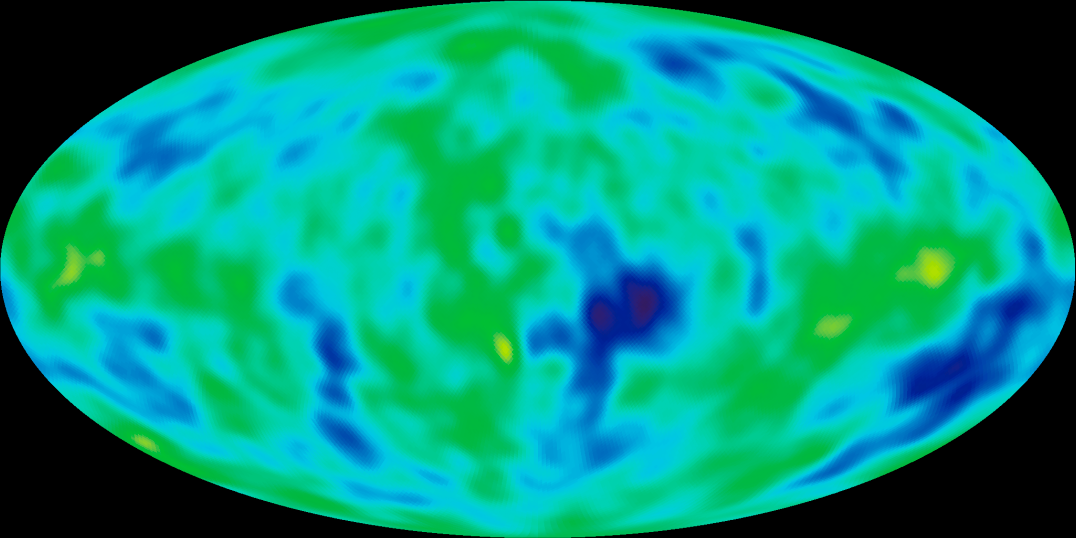
\includegraphics[width=\textwidth]{Images/COBE.png}
    }
    \only<14-14>{%
      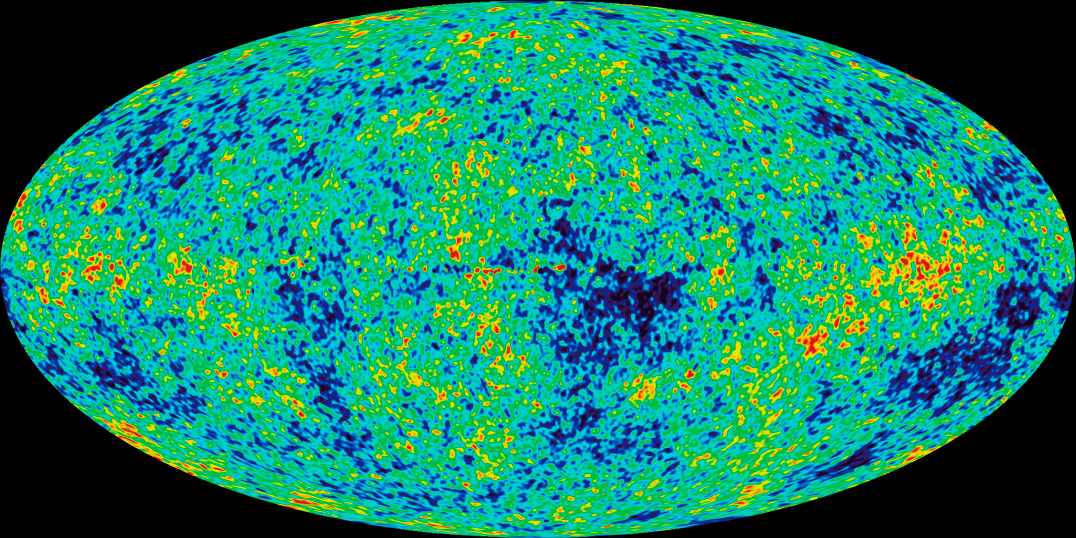
\includegraphics[width=\textwidth]{Images/wmap.png}
    }
    \only<15-15>{%
      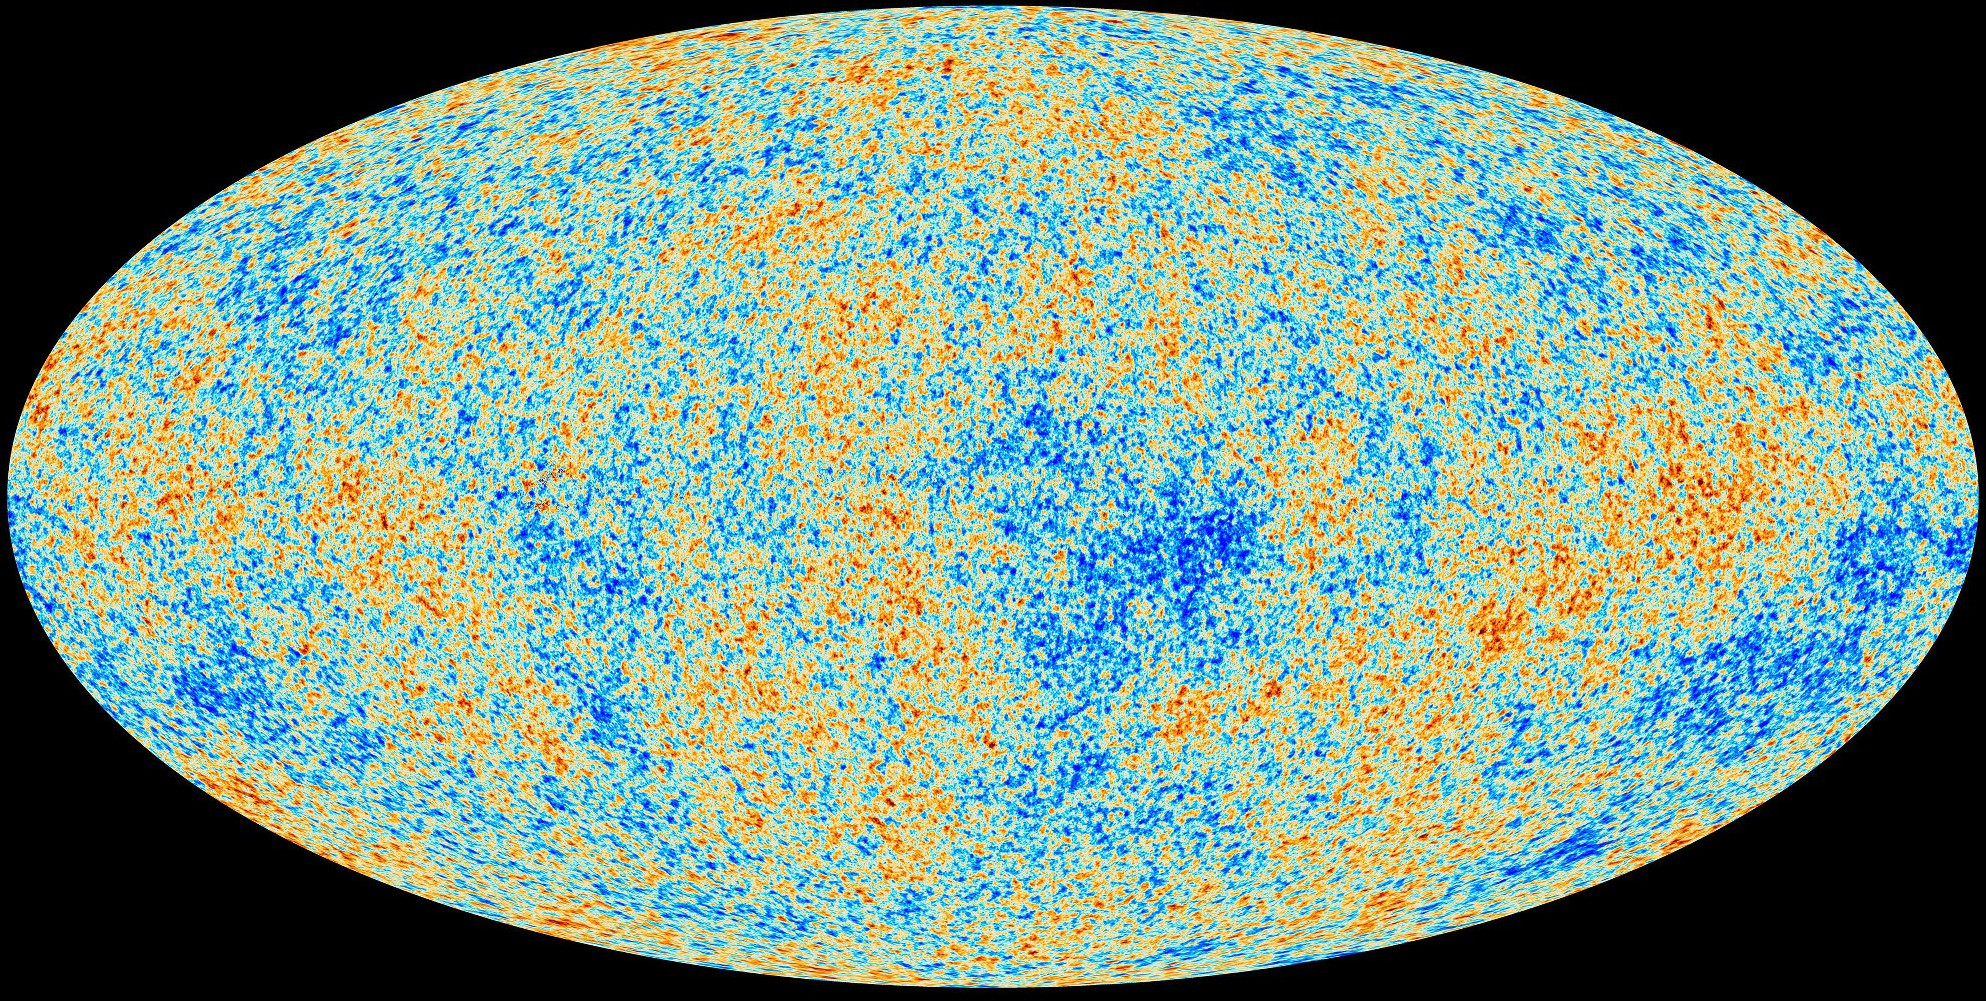
\includegraphics[width=\textwidth]{Images/planckdata.jpg}
    }

    \only<2-4>{%
    \begin{itemize}
      \only<2-3>{\item Map of the earth}
      \only<4>{\item Map of the sky}
    \end{itemize}
  }

    \only<6-9>{%
    \begin{itemize}
      \only<6-9>{\item `Subtract off' the constant source.}
      \only<8-9>{\item COBE microwave satellite (1992)}
      \only<9>{\item These direction-dependent deviations are called {\em Anisotropies} }
    \end{itemize}
  }

    \only<10-12>{%
    \begin{enumerate}
      \only<10-12>{\item Galaxy in the middle}
      \only<11-12>{\item One half hotter than the other}
      \only<12-12>{\item Additional fluctuations}
    \end{enumerate}
  }

  \only<13>{%
    \begin{itemize}
      \only<13>{\item COBE (1992)}
    \end{itemize}
  }

  \only<14>{%
    \begin{itemize}
      \only<14>{\item WMAP (2001--2010)}
    \end{itemize}
  }

  \only<15>{%
    \begin{itemize}
      \only<15>{\item Planck (2009--2013)}
    \end{itemize}
  }

  \end{overlayarea}

\end{frame}

